\chapter{Finite element method: formulation}

\disclaimer

\section{Introduction}
The objective of this section is threefold.  We first introduce finite elements for reference triangles. We then discuss the assembly of finite elements to construct a finite element space.  We finally discuss approximation properties of these finite element spaces.

\section{Triangulation}
We first introduce a \emph{triangulation} of $\Omega \subset \RR^d$.  A triangulation
\begin{equation*}
  \calT_h \equiv \{ K_i \}_{i=1}^{n_e}
\end{equation*}
is a set of non-overlapping elements $K_1, \dots, K_{n_e}$ such that union of the closure of the elements cover the domain: $\cup_{i=1}^{n_e} \overline K_i = \overline \Omega$.   (We consider the closure of the elements because we consider each element to be open.) An example of triangulation of a square domain $\Omega$ is shown in Figure~\ref{fig:fe_mesh_p1}. The triangulation comprise $n_e = 9$ triangular elements, which are delineated by $n_v = 9$ vertices.  The subscript $h$ of the triangulation $\calT_h$ signifies the maximum diameter of the elements in the triangulation; specifically, $h \equiv \max_{i} \text{diam}(K_i)$, where $\text{diam}(K_i)$ is the diameter of the smallest ball that inscribes the element $K_i$.  Intuitively (and as we will see more formally), the finite element spaces associated with a sequence of triangulations get richer as $h$ decreases.  In general, a triangulation comprises line segments in one dimension, triangles or quadrilaterals in two dimension, and tetrahedrons or hexahedrons in three dimensions.


\begin{figure}
  \centering
  \subfigure[mesh]{
    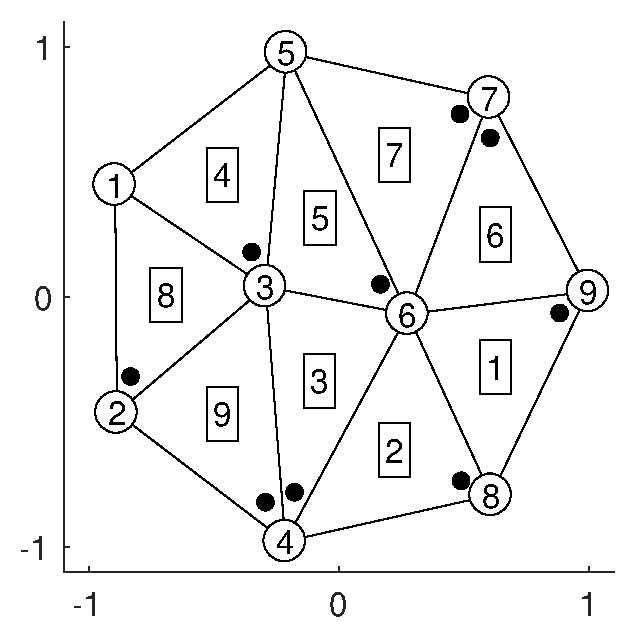
\includegraphics[width=0.4\textwidth]{fe_mesh_p1}
  }
  \caption{Triangulation.}
  \label{fig:fe_mesh_p1}
\end{figure}

While mathematically a triangulation is simply a collection of non-overlapping elements, we need a convenient means to represent the triangulation on a computer.  One approach is to store tables of \emph{node coordinates} and \emph{element-node connectivities}.  Tables~\ref{tb:fe_mesh_p1_coord} and \ref{tb:fe_mesh_p1_tri} are respectively the coordinate and connectivity tables associated with the triangulation shown in Figure~\ref{fig:fe_mesh_p1}. The connectivity table indicates that, for instance, element 5 is delineated by the nodes 6, 5, and 3; the coordinate table then indicates that the coordinates of these three nodes are $(0.28,-0.07)$, $(-0.21,0.98)$, and $(-0.29,0.04)$, respectively.  Note that, in Figure~\ref{fig:fe_mesh_p1}, for each triangle, we indicate the first of the three nodes that delineate the triangle by a dot ($\bullet$); with this convention we have identical information presented in Figure~\ref{fig:fe_mesh_p1} in a visual form and Tables~\ref{tb:fe_mesh_p1_coord} and \ref{tb:fe_mesh_p1_tri} in an array form.

\begin{table}
  \centering
  \subfigure[coordinates]{
    \begin{tabular}{c|cc}
      node & $x_1$ & $x_2$ \\
      \hline
      $1$ & $-0.89$ & $\hphantom{-}0.45$ \\ 
      $2$ & $-0.89$ & $-0.46$ \\ 
      $3$ & $-0.29$ & $\hphantom{-}0.04$ \\ 
      $4$ & $-0.21$ & $-0.98$ \\ 
      $5$ & $-0.21$ & $\hphantom{-}0.98$ \\ 
      $6$ & $\hphantom{-}0.28$ & $-0.07$ \\ 
      $7$ & $\hphantom{-}0.60$ & $\hphantom{-}0.80$ \\ 
      $8$ & $\hphantom{-}0.61$ & $-0.79$ \\ 
      $9$ & $\hphantom{-}1.00$ & $\hphantom{-}0.02$ \\ 
    \end{tabular}
    \label{tb:fe_mesh_p1_coord}
  }
  \subfigure[connectivity]{
    \begin{tabular}{c|ccc}
      element & node 1 & node 2 & node 3 \\
      \hline
      $1$ & $9$ & $6$ & $8$ \\ 
      $2$ & $8$ & $6$ & $4$ \\ 
      $3$ & $4$ & $6$ & $3$ \\ 
      $4$ & $3$ & $5$ & $1$ \\ 
      $5$ & $6$ & $5$ & $3$ \\ 
      $6$ & $7$ & $6$ & $9$ \\ 
      $7$ & $7$ & $5$ & $6$ \\ 
      $8$ & $2$ & $3$ & $1$ \\ 
      $9$ & $4$ & $3$ & $2$ \\ 
    \end{tabular}
    \label{tb:fe_mesh_p1_tri}
  }
  \caption{Node coordinate and connectivity table for mesh shown in Figure~\ref{fig:fe_mesh_p1}.}
  \label{tb:fe_mesh_p1}
\end{table}

The task of generating a triangulation for a given domain is called \emph{mesh generation} and a program that carries out the task is called a \emph{mesh generator} or \emph{mesher}.  Mesh generation is a non-trivial task.  In fact, the development of algorithms that can robustly and automatically generate high-quality triangulation for complex geometries in three dimensions is an area of ongoing research.  Nevertheless, because mesh generation is essential for any finite element discretization, there is a large number of commercial and open-source meshers.  Here we name a few user-friendly, open-source meshers:
\begin{itemize}
\item \texttt{triangle}. A robust two-dimensional mesher written in C that generates meshes with a guaranteed quality certificate in terms of the minimal angle.
\item \texttt{tetgen}. A popular three-dimensional mesher written in C.
\item \texttt{distmesh}.  A user-friendly mesher written in \textsc{Matlab} for implicit domain geometries represented by level sets. 
\end{itemize}
The mesh shown in Figure~\ref{fig:fe_mesh_p1} was in fact generated by \texttt{distmesh}.  We will extensively use \texttt{distmesh} to generate meshes in this course as it is implemented in \textsc{Matlab} and is easy to use.


\section{Approximation spaces}
We now introduce piecewise polynomial spaces associated with the triangulation $\calT_h$:
\begin{equation*}
  \calV_h \equiv \{ v \in \calV \ | \ v|_K \in \PP^p(K), \ K \in \calT_h \},
  \label{eq:fe_Vh}
\end{equation*}
where $\PP^p(K)$ is the space of polynomials of degree at most $p$ over $K$.  We note the two requirements: $v \in \calV_h$ must belong to $\calV$ and in particular satisfy the essential boundary conditions; $v$ restricted to any element $K$, $v|_K$, must be a polynomial of degree $p$. Figure~\ref{fig:fe_fun_p1} shows an example of a function in a linear finite element space,
\begin{equation*}
  \calV_h \equiv \{ v \in \calV \equiv H^1(\Omega) \ | \ v|_K \in \PP^1(K), \ K \in \calT_h \},
  \label{eq:fe_lin_Vh}
\end{equation*}
associated with the mesh shown in Figure~\ref{fig:fe_mesh_p1}.

\begin{figure}
  \centering
  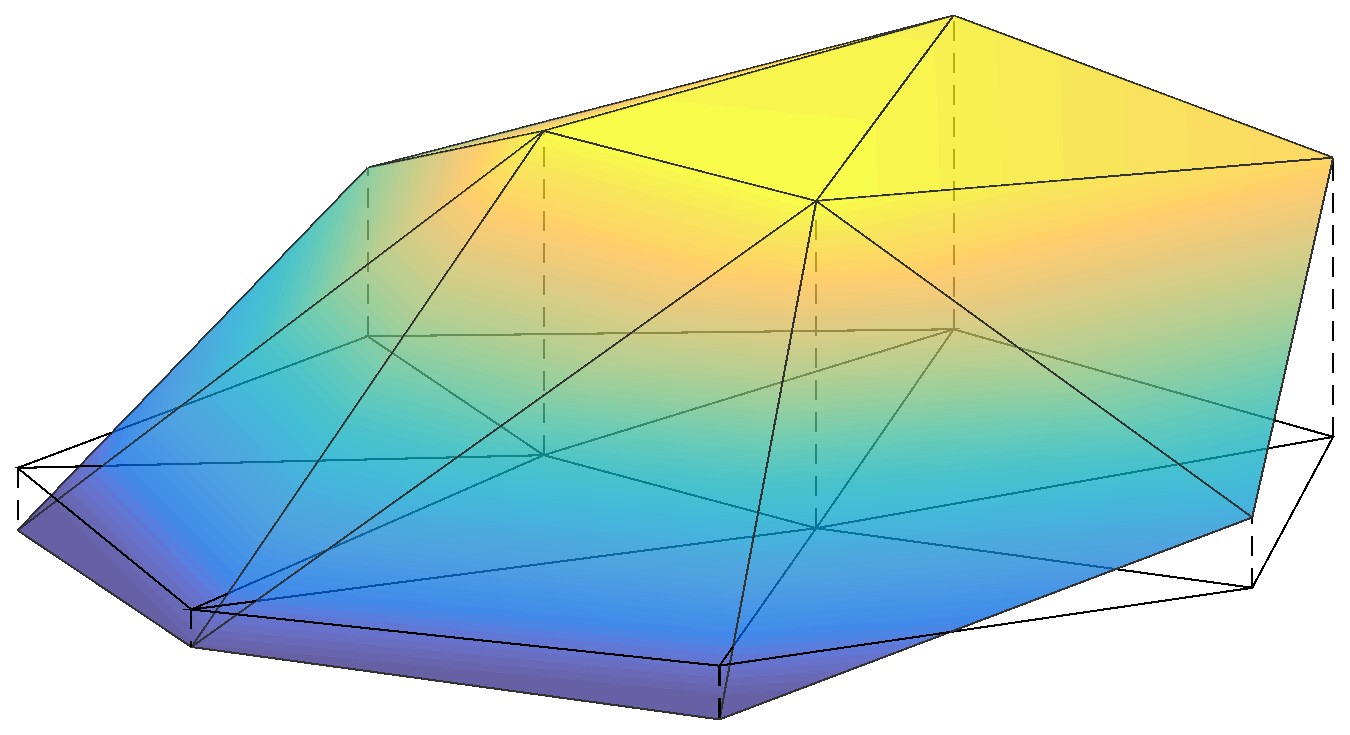
\includegraphics[width=0.45\textwidth]{fe_fun_p1}
  \caption{A function in a linear finite element space.}
  \label{fig:fe_fun_p1}
\end{figure}

We note that the condition $\calV_h \subset \calV \subset H^1(\Omega)$ implies that the function must be continuous across element interfaces.  If a function is continuous and piecewise polynomial, the (distributional) derivative is piecewise polynomial and hence is in square integrable (i.e., in $L^2(\Omega)$); the function hence is in $H^1(\Omega)$.  If a function is not continuous across element interfaces, then (distributional) derivative generates delta distributions at the interfaces and hence is not in $L^2(\Omega)$. In fact, for a piecewise polynomial space, the continuity is the necessary and sufficient condition for the function to be in $H^1(\Omega)$. 

We now need a convenient means to describe functions in $\calV_h$ given by~\eqref{eq:fe_lin_Vh}, such as the one shown in Figure~\ref{fig:fe_fun_p1}.  Specifically, we need to pick \emph{global degrees of freedom} with which we can uniquely describe any function in $\calV_h$. To this end, we introduce a \emph{basis} for the linear space $\calV_h$.  We recall that a set of functions $\{ \phi_i \}_{i=1}^n$ is a basis for $\calV_h$ if the set (i) spans $\calV_h$ and (ii) is linearly independent. The first requirement implies that any $w \in \calV_h$ can be expressed as a linear combination of $\{ \phi_i \}_{i=1}^n$.  The second requirement implies that the coefficients associated with the representation of $w \in \calV_h$ in terms of $\{ \phi_i \}_{i=1}^n$ is unique.  In other words, if $\{ \phi_i \}_{i=1}^n$ is a basis for $\calV_h$, then for any given $w \in \calV_h$ there exists a unique $\hat w \in \RR^n$ such that
\begin{equation*}
  w = \sum_{j=1}^n \hat w_j \phi_j,
\end{equation*}
where $n = \text{dim}(\calV_h)$.

While the choice of a basis is not unique, one convenient choice is a \emph{Lagrange basis} or \emph{nodal basis}.  Nodal basis comprises functions that take on the value of 1 at the associated node and 0 at all other nodes:
\begin{equation}
  \phi_j(x_i) = \delta_{ij},
  \label{eq:fe_lagrange_basis_prop}
\end{equation}
where $\delta_{ij}$ is the Kronecker delta so that $\delta_{ij} = 1$ if $i = j$ and $\delta_{ij} = 0$ if $i \neq j$. Figure~\ref{fig:fe_mesh_p1} shows an example of basis function, $\phi_3$, for the linear finite element space associated with the mesh shown in Figure~\ref{fig:fe_mesh_p1}.  For the linear finite element space $\calV_h$ defined by~\eqref{eq:fe_lin_Vh}, there are 9 nodal basis functions, one associated with each node.  We also observe that the set of the 9 functions indeed forms a basis: the set is linearly independent and spans the space. The set is linearly independent because $\sum_{j=1}^n \hat w_j \phi_j = 0$ implies $\sum_{j=1}^n \hat w_j \phi_j(x_i) = 0$, $\forall i =1,\dots,n$, which in turn implies $\hat w_j = 0$, $j = 1,\dots,n$.  The set spans the space because the piecewise linear polynomial space is 9 dimensional and the linearly independent set contains 9 functions.

\begin{figure}
  \centering
  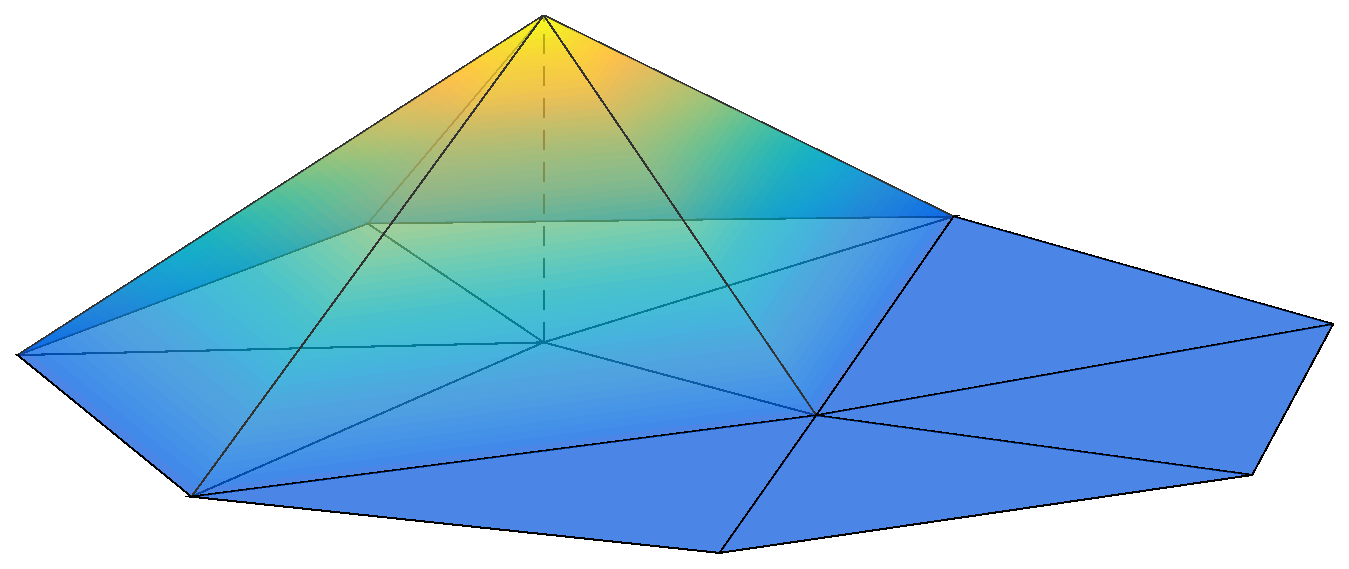
\includegraphics[width=0.48\textwidth]{shape_global_p1}
  \caption{Nodal basis $\phi_3$ for the linear finite element space $\calV_h$ defined by \eqref{eq:fe_lin_Vh}.}
  \label{fig:fe_shape_global_p1}
\end{figure}

While the choice of basis not unique, the nodal basis provides a convenient interpretation in the physical space.  Specifically, for $w \in \calV_h$, we have a (unique) representation
\begin{equation}
  w(x) = \sum_{j=1}^n \hat w_j \phi_j(x) = \sum_{j=1}^n w(x_j) \phi_j(x).
  \label{eq:fe_rep}
\end{equation}
We note that the coefficient $w_j$ must be equal to $w(x_j)$, because $w(x_i) = \sum_{j=1}^n \hat w_j \phi_j(x_i) = \sum_{j=1}^n \hat w_j \delta_{ij} = w_i$, $i = 1,\dots,n$; here, the second equality follows from the Lagrange interpolation property~\eqref{eq:fe_lagrange_basis_prop}.  In words, $w_j = w(x_j)$, the value of the function $w \in \calV_h$ evaluated at the associated node $x_j$. This interpretation of nodal basis allows us to readily confirm that the nodal basis are indeed basis: for any $w \in \calV_h$, there exists a unique $\hat w \in \RR^n$ such that $w = \sum_{j=1}^n \hat w_j \phi_j$.  We can clearly express any function $w \in \calV_h$ in the form~\eqref{eq:fe_rep}; moreover the representation is unique. 

\section{Finite element approximation}
We now week a finite element approximation.  

\section{Minimization formulation: Rayleigh-Ritz}
We now seek the finite element approximation to the problem using the minimization formulation. To this end, we recall that the energy functional is given by 
\begin{align*}
  J(w) =  J(\sum_{j=1}^n \hat w_j \phi_j)
  = \frac{1}{2} a (\sum_{j=1}^n \hat w_j \phi_j, \sum_{i=1}^n \hat w_i \phi_i) - \ell(\sum_{i=1}^n \hat w_i \phi_i)
  = \frac{1}{2} \sum_{i,j=1}^n \hat w_i a(\phi_j,\phi_i) \hat w_j - \sum_{i=1}^n \hat w_i \ell(\phi_i)
\end{align*}

\begin{equation*}
  (\hat A_h)_{ij} \equiv a(\phi_j,\phi_i)
  \quad \text{and} \quad
  (\hat f_h)_i \equiv \ell(\phi_i)
\end{equation*}

\begin{equation*}
  \hat J(\hat w) = J(\sum_{j=1}^n \hat w_j \phi_j)
  = \frac{1}{2} \hat w^T \hat A_h \hat w - \hat w^T \hat f_h
\end{equation*}

\begin{equation*}
  \hat u_h = \argmin_{\hat w \in \RR^n} \hat J(\hat w)
\end{equation*}

\begin{equation*}
  \nabla \hat J(\hat u_h) = \hat A_h \hat u_h - \hat f_h = 0
\end{equation*}
